% Created 2013-03-02 Sat 23:14
\documentclass[a4paper,11pt]{article}
\usepackage[utf8]{inputenc}
\usepackage[T1]{fontenc}
\usepackage{fixltx2e}
\usepackage{graphicx}
\usepackage{longtable}
\usepackage{float}
\usepackage{wrapfig}
\usepackage{soul}
\usepackage{textcomp}
\usepackage{marvosym}
\usepackage{wasysym}
\usepackage{latexsym}
\usepackage{amssymb}
\usepackage{hyperref}
\tolerance=1000
\usepackage{fontspec}
\usepackage[titletoc,page,title]{appendix}
\usepackage{biblatex}
\usepackage{metalogo}
\usepackage{graphicx}
\bibliography{fyp}
\defaultfontfeatures{Mapping=tex-text}
\setromanfont[Ligatures={Common},Numbers={Lining}]{Linux Libertine}
\providecommand{\alert}[1]{\textbf{#1}}

\title{A Weighted Least Squares Method for Time Delay Estimation in Gravitationally Lensed Photon Streams}
\author{\Large{Micha{\l} Staniaszek} \\\small{Supervisor: Peter Tiňo}}
\date{\today}
\hypersetup{
  pdfkeywords={},
  pdfsubject={},
  pdfcreator={Emacs Org-mode version 7.8.11}}

\begin{document}

\maketitle


\thispagestyle{empty}
\newpage
\pagenumbering{roman}
In this report, we present a system for the estimation of the time delay $\Delta
t$ between multiple realisations of a Poisson process with the underlying
function $\lambda(t)$, with particular application to gravitationally lensed
photon streams. We build on the weighted least squares approach to develop a
linear estimator which we use to estimate $\lambda(t)$. We then introduce a
numerical and probabilistic method for estimating $\Delta t$ using the function
estimates. Finally, we compare the performance of our linear estimator to kernel
regression on simulated data and data from real quasars.

\vspace{1.0cm}\textbf{Keywords: }Poisson process, gravitational lensing,
 machine learning, linear estimation

\begin{center}
\vspace*{\fill}\scriptsize{Typeset in Linux Libertine using \XeLaTeX}.
\end{center}
\newpage
\tableofcontents
\newpage
\pagenumbering{arabic}
\section{Introduction}
\label{sec-1}

With continued advances in computing and sensing technologies, the amount of
data that can be gathered from both everyday objects and scientific experiments
has increased rapidly. However, more data is not always a blessing---it must be
stored and analysed for it to have any use, and this is not an easy task when
one has terabytes of data to deal with. The Large Hadron Collider at CERN is one
perhaps extreme example, producing on the order of five terabytes of data each
second. Storing this amount of data, let along analysing it is impossible, and
so multiple stages of intelligent filtering are applied, reducing the throughput
to 100 gigabytes per second, and then further to around 200 megabytes per
second, where it is finally stored, producing almost two CDs each second
\cite{WLCGproc}. This project focuses on creating the foundations for a system
to do such intelligent filtering, but in the context of astronomical data. The
volume of data produced by modern telescopes, while not on the same scale as the
LHC, is nonetheless overwhelming. Image sizes of one to two gigabytes are not
uncommon, and deciding what data is actually relevant is not a trivial task
\cite{starck2002handbook}. Using intelligent filtering algorithms, it should be
possible to flag up interesting-looking data for further study. While there are
many areas in which such capabilities would be useful, we are particularly
interested in finding candidates for images of gravitationally lensed
objects. In order to do this, it is necessary to find pairs of observations of
photon flux which appear to have the same underlying function. More precisely,
given a set of data containing the time of arrival of photons from a particular
source, henceforth called a \emph{stream}, we wish to find another stream which,
when shifted in time by some value $\Delta$, has similar numbers of photons
arriving in a given interval as the first stream. We call $\Delta$ the
\emph{delay} between the two streams. In this project, we develop a system which
can generate simulated photon streams using Poisson processes, use linear
regression to estimate the underlying function of a given stream, and, given the
function estimates of two streams, estimate the time delay between them. Knowing
the value of the time delay has many applications in astrophysics, and with more
precise estimates, more accurate calculations can be made to increase our
understanding of the universe we live in.

In section \ref{sec-2} we discuss the concepts underpinning the project in more
detail, with a more in-depth explanation of the issues surrounding the
calculation of the time delay and its uses. In section \ref{sec-3} we introduce our method of generating photon streams from Poisson
processes. Section \ref{sec-4} shows our approach to estimating the
underlying function of a given stream of photons. Our methods of calculating the
time delays between multiple photon streams are explained in section \ref{sec-5}. Section \ref{sec-6} gives detailed information on the design and
development of the system, including the software and project management
aspects. Finally, in section \ref{sec-7} we present experimental data from both
simulated and real data and discuss the relative effectiveness of our methods.
\section{Background}
\label{sec-2}
\subsection{Gravitational Lensing}
\label{sec-2-1}

In an eight-year period starting in 1907 and ending in 1915 with the publication
of a paper on field equations of gravitation\cite{einstein1915general}, Albert
Einstein wrote many papers developing a new theory of gravitation, his general
theory of relativity. This generalisation of special relativity and Newton's law
of universal gravitation led to a revolution in the field of physics, and
remains one of the most important scientific discoveries to date. The theory
describes how spacetime is affected by the presence of matter and radiation, and
this idea has many important consequences, but one of the effects in particular
is important in the context of this report.

According to the theory, objects with mass, or massive objects, cause spacetime
to curve around them. A simple way to visualise this effect is to imagine
dropping a ball onto a sheet of cloth which has been pulled taut. The ball will
eventually come to a stop in the centre of the cloth, and cause it to sag. Here,
the sheet represents spacetime, and the ball represents anything from planets,
to stars, or even entire galaxies. Depending on the weight of the ball, the
shape of the cloth will be affected to different degrees---a ping pong ball will
have hardly any effect at all, but if we drop a bowling ball onto the sheet, the
effect will be significant. In a similar way, the amount that spacetime curves
around a massive object depends on its mass. An object with high mass will cause
a large amount of curvature, whereas a lower mass object will cause less. If a
second ball, lighter than the first, is introduced to the system, what happens?
With no initial velocity, it will roll in a straight line towards the first ball
sitting at the centre of the sheet. This is one way of thinking about gravity
and its relationship with spacetime---an object's gravitational attraction is a
result of its mass curving spacetime, and the strength of the attraction is
proportional to the mass. While objects with no mass, such as photons, cannot be
affected by gravity directly, they \emph{are} affected by the curvature of
spacetime. This bending of light rays is known as
\emph{gravitational lensing}.

\begin{figure}
\centering
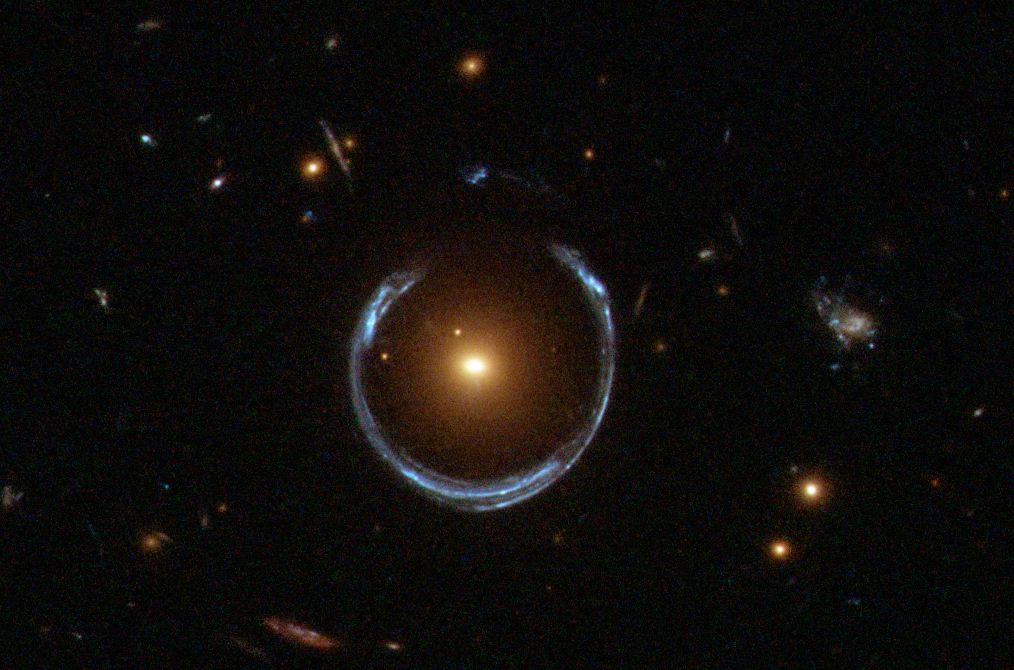
\includegraphics[width=\textwidth]{einstein_ring}
\caption{An example of a gravitational lensing effect known as an Einstein ring.
In this image, the central galaxy, LRG 3-757, is distorting light from a distant
blue galaxy \cite{einsteinring}.}
\label{fig:einsteinring}
\end{figure}
\begin{itemize}
\item what is it
\item how does it occur
\item pictures
\item what does it tell us about the universe or things in it
\end{itemize}
\subsubsection{Importance of the Time Delay}
\label{sec-2-1-1}

\begin{itemize}
\item Talk generally about the problem of time delay estimation
\item refer to physics papers attempting to make estimates of the delay
\item talk about time delay estimation in particular, refer to kundic et al, many others
\item talk about how better estimates benefit the scientific community
\item refer to peter's paper about the efficacy of kernel regression
\item better estimators are necessary to increase the accuracy of estimates
\item this is an experiment to see whether this method has any use
\item build on technique introduced in massey et al
\end{itemize}
\subsection{Poisson Processes}
\label{sec-2-2}

\begin{itemize}
\item where do they occur
\item what can they be used for
\item Times for a homogeneous poisson process can be generated using
     the formula $\log\frac{-U}{\lambda}$
\end{itemize}
\subsection{Linear Regression}
\label{sec-2-3}
\section{Simulation of Photon Streams}
\label{sec-3}
\subsection{Function Generation}
\label{sec-3-1}
\subsection{Generating Streams from Functions}
\label{sec-3-2}
\section{Function Estimation}
\label{sec-4}
\subsection{Baseline Estimation}
\label{sec-4-1}
\subsubsection{Optimum Least Squares}
\label{sec-4-1-1}
\subsubsection{Iterative Weighted Least Squares}
\label{sec-4-1-2}
\subsubsection{Piecewise Iterative Weighted Least Squares}
\label{sec-4-1-3}

    Initially, we thought that it may be possible to decide whether to
    extend the line or not based on the difference in slope between
    the estimate from the previous time interval and the estimate of
    the next. If the previous estimate was positive, and the next
    negative, and vice versa, clearly the line should not be
    continued. The intercept parameter was considered to be much less
    important. However, this assumption was highly flawed. Due to the
    nature of poisson processes, it is perfectly possible that
    although the function has changed significantly after the end of
    the previous interval, the estimate for the interval that we are
    trying to extend the line into could return very similar values to
    that of the previous interval. Because of this, we extend the line
    when we should not be doing so. There are several potential
    solutions to this problem. First, rather than forming a new
    estimate, we extend the line and then check how much the error has
    increased. If it goes over a certain threshold, then we reject the
    extension attempt and try again, this time with a shorter
    extension. Another potential way of improving the piecewise
    estimation in general would be to require the estimate for the
    next time period to start from the end point of the last time
    period. This would prevent the intercept parameter from changing,
    and would force the estimator to find the best estimate given a
    specific starting point, rather than giving it free reign to find
    the estimate which actually minimises the error.
\begin{itemize}

\item coding issues\\
\label{sec-4-1-3-1}%
what to do with the issue of minimum length of intervals? Sometimes
not extending the original gives a better estimate of the line than
re-estimating the interval extended, or adding the short interval onto
the end of the previous one and using its estimate. See data in the
min$_{\mathrm{interval}}$$_{\mathrm{length}}$ folder in data. The better fitting line is the
baseline estimate of that with no minimum, and the other set is the
estimate with minimum interval length applied
\end{itemize} % ends low level
\subsubsection{Baseline}
\label{sec-4-1-4}
\subsection{Kernel Density Estimation}
\label{sec-4-2}
\section{Time Delay Calculation}
\label{sec-5}
\subsection{Area Method}
\label{sec-5-1}
\subsection{Probability Mass Function Method}
\label{sec-5-2}
\section{System}
\label{sec-6}
\subsection{System Structure}
\label{sec-6-1}
\subsubsection{Overall Structure}
\label{sec-6-1-1}
\subsubsection{Estimators}
\label{sec-6-1-2}
\subsubsection{Generators}
\label{sec-6-1-3}
\subsubsection{Experimenter}
\label{sec-6-1-4}
\subsection{Development}
\label{sec-6-2}
\subsubsection{Development Process}
\label{sec-6-2-1}
\subsubsection{Version Control}
\label{sec-6-2-2}

\begin{itemize}
\item branching strategy
\item commit frequency
\item using issues on github
\end{itemize}
\subsubsection{Project Management}
\label{sec-6-2-3}

\begin{itemize}
\item keep changelog
\item writing up and planning layout in notebook
\end{itemize}
\section{Evaluation}
\label{sec-7}
\subsection{experimentation on simulated data}
\label{sec-7-1}
\subsection{experimentation on real-world data}
\label{sec-7-2}
\section{Conclusion}
\label{sec-8}

\newpage
\nocite{*}
\printbibliography
\newpage
\section{Installation}
\label{sec-9}
\subsection{MuParser}
\label{sec-9-1}

 download package\\
 run \texttt{./configure --prefix=/usr}, followed by \texttt{make \&\& make install} (may require sudo)
 this installs muparser so that headers can be found in \texttt{/usr/include}
    
    sudo apt-get install libgsl0-dev check 

\end{document}